\documentclass[]{article}

% Packages
\usepackage[nottoc,notlof,notlot]{tocbibind} 
\usepackage[margin=1in]{geometry}
\usepackage{changepage}
\usepackage{graphicx}
\usepackage{caption}
\usepackage{subcaption}
\usepackage{hyperref}
\usepackage{fancyhdr}
\usepackage{titletoc}
\usepackage [english]{babel}
\usepackage [autostyle, english = american]{csquotes}
\usepackage{lmodern}
\usepackage{sectsty}

% User def
%\textsuperscript{\cite{ref:1}}
%	\begin{figure}[h]
%	\centering
%	\begin{subfigure}{.5\textwidth}
%		\centering
%		%\includegraphics[width=.7\linewidth]{img/BefunExec_ESG_example.png}
%		\caption{Stack trace of program}
%		\label{fig:BefunTrace}
%	\end{subfigure}%
%	\begin{subfigure}{.5\textwidth}
%		\centering
%		%\includegraphics[width=0.7\linewidth]{img/BefunExec_ESH_example.png}
%		\caption{How the stack is utilised}
%		\label{fig:BefunStack}
%	\end{subfigure}
%	\caption{Befunge program running a program with stack visualisation}
%	\label{fig:Befunge}
%\end{figure}

% Set formats for each heading level


% Page Style
\pagestyle{fancy}
\fancyhf{}
\fancyhead[L]{Architectural Requirements}
\fancyhead[C]{}
\fancyhead[R]{Last revised: 10 August 2017}
\renewcommand{\headrulewidth}{0.4pt}
\fancyfoot[L]{Code 9}
\fancyfoot[C]{}
\fancyfoot[R]{Page \thepage}
\renewcommand{\footrulewidth}{0.4pt}

\sectionfont{\fontfamily{lmss}\selectfont}
\subsectionfont{\fontfamily{lmss}\selectfont}
% TOC levels
\setcounter{tocdepth}{4}
\setcounter{secnumdepth}{4}

% Title Page
\begin{document}\thispagestyle{empty}\fontfamily{lmss}\selectfont	
	\tableofcontents
	\clearpage
	
	\addcontentsline{toc}{section}{Architectural Requirements}
	\section*{Architectural Requirements}
		\begin{adjustwidth}{2.5em}{0pt}
			\addcontentsline{toc}{subsection}{\protect\numberline{}Introduction}
			\subsection*{Introduction}
			\begin{flushleft}
				The system design to be implemented will be referred to as a Hybrid-tier System. This hybrid model is based off the n-tier (multi-layered) architecture, where the system is divided into layers. This multi-layered system is also referred to as a Client-Sever architecture. For this architecture, there are four tiers/layers. Those being: 
				\begin{enumerate}
					\item Presentation Tier
					\item Server Tier
					\item Database Tier
					\item AI (Artificial Intelligence) Algorithm Tier
				\end{enumerate}
				 Each layer will be modifiable without needing to change the entire application. As a result of the aforementioned, maintenance and adding extra functionality is easier. Overall complexity of code over all layers will be reduced, thus making the layers reusable in other applications. Since the layers do not act like a traditional n-tier where one would delegate tasks to other layers; once a request goes to the server tier, the server will decide if it will go to the database tier or the AI tier which then goes to the database tier. Thus showing an optimised parallel system to deal with requests.
				 Additionally, the use of this architecture system will allow different members of our team to modify separate layers without interference. It is possible to deploy each layer (specifically the database and server layers) over multiple locations for better reliability and performance. What differentiates the hybrid architecture from a traditional n-tier or client-server, is in how the layers are implemented. Figure \ref{fig:Deployment} shows the overall architecture of this hybrid system.
				 	\begin{figure}[h]
					 	\centering
				    	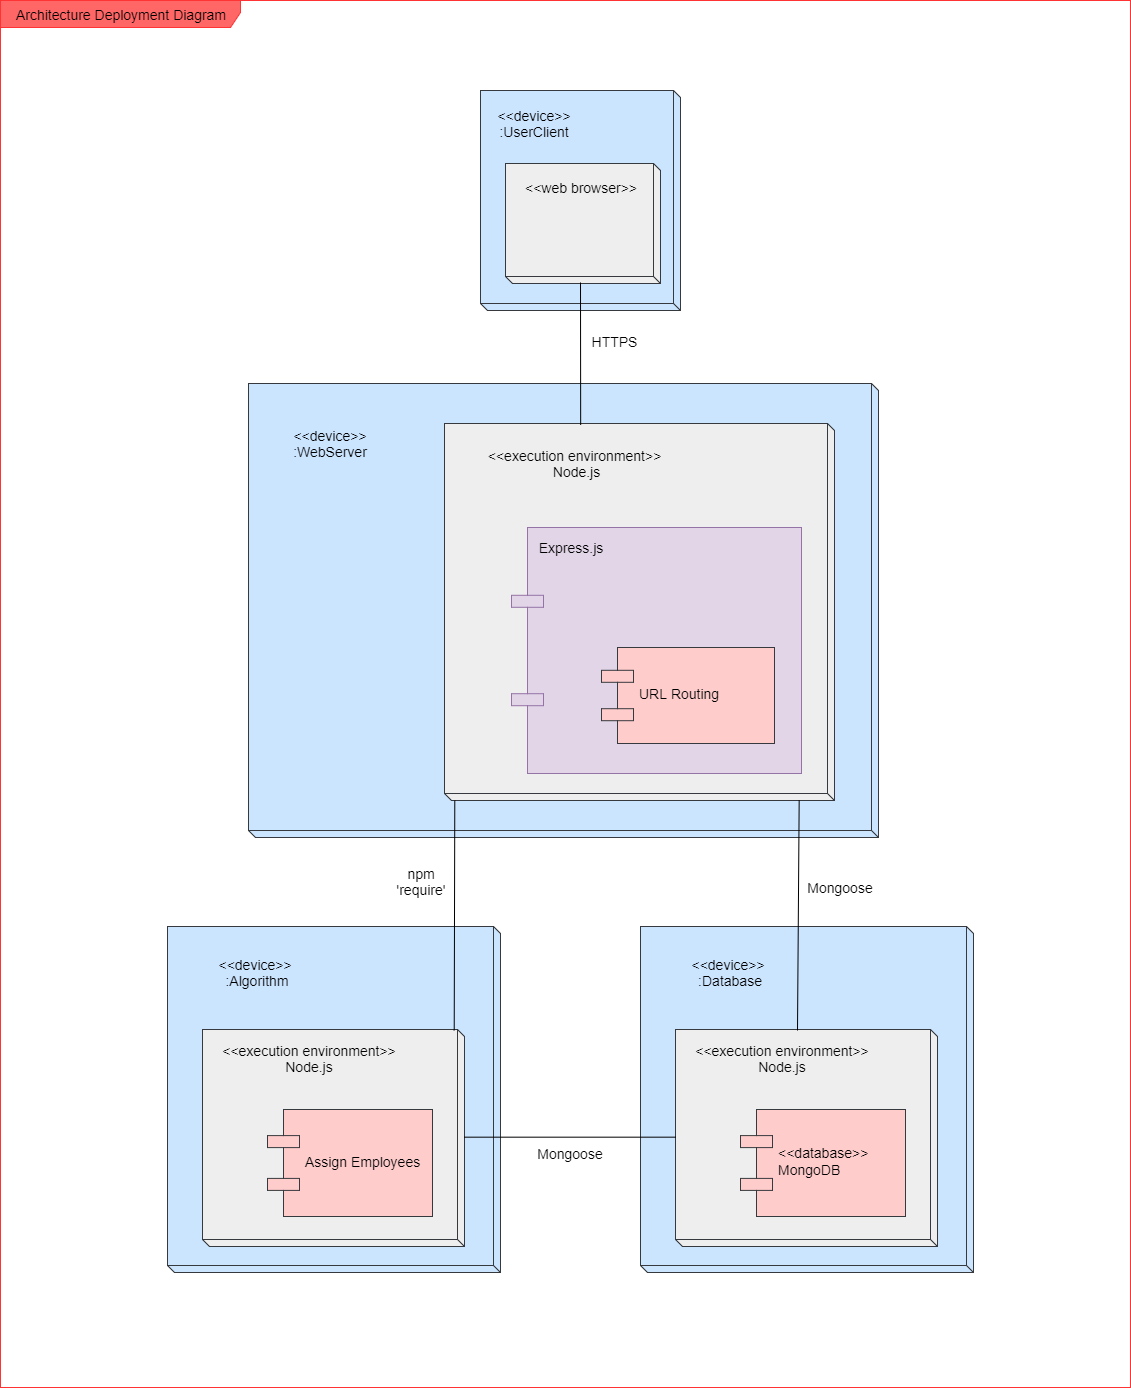
\includegraphics[width=0.56\linewidth]{Diagrams/deployment.png}
					 	\caption{Deployment Diagram: Hybrid-Tier Architecture}
					 	\label{fig:Deployment}
				 	\end{figure}
			\end{flushleft}
		
			\addcontentsline{toc}{subsection}{\protect\numberline{}Presentation Tier}
			\subsection*{Presentation Tier}
			\begin{flushleft}
			This is the layer the user will be interacting with. It encompasses the actual applications that can be developed (Android, iOS and web), and any interactions that the users may have with them. In this system, the user will primarily work with a web application as the front-end.
			\newline 
			
			\textbf{The presentation tier includes:}
			\begin{itemize}
				\item Displaying the user interface (UI), which the user will interact with. 
				\item Adding notification, forms, buttons and pages. 
				\item Providing an interface to trigger requests to the system. 
				\item Ultimately serving as a communication medium between pages on the front-end, and to send and receive data between the back-end.
			\end{itemize}
			\end{flushleft}
	
			\addcontentsline{toc}{subsection}{\protect\numberline{}Server Tier}
			\subsection*{Server Tier}
			\begin{flushleft}
			The server layer implements the business logic, and process all requests made by the front-end - it makes logical decisions based on the interactions from the presentation layer and then decides what or where data needs to go; either to the database layer or the AI layer.
			\newline
			
			\textbf{The server tier is responsible for:}
			\begin{itemize}
				\item Allow admin users to be able to add/remove/edit client projects, and assign employees to specific projects.
				\item Automatically update calendars of employees.
				\item Crosscheck projects before assigning them to an employee.
				\item Server communication over the internet.
				\item Scheduling Assistant calculations. 
				\item Limit an employee from being able to edit projects they have been assigned to.
				\item Allow an employee to add other events to his/her calendar if these do not clash with the pre-populated events.
				\item Session management.
			\end{itemize}
			\end{flushleft}

			\addcontentsline{toc}{subsection}{\protect\numberline{}Database Tier}
			\subsection*{Database Tier}
			\begin{flushleft}
				The data layer is where the information used by the presentation layer for sending and retrieving, is stored. This layer consists of:
				\begin{itemize}
					\item Recommended time slots where all employees are available. 
					\item Server storage with MongoDB
					\item View individual employee calendar and assigned projects. 
				\end{itemize}
			\end{flushleft}
		
			
			\addcontentsline{toc}{subsection}{\protect\numberline{}AI (Artificial Intelligence) Algorithm Tier}
			\subsection*{AI (Artificial Intelligence) Algorithm Tier}
			\begin{flushleft}
			    The AI layer houses the resource allocation algorithm, and is used by the server layer to allocate employees to a project. This layer runs off its own independent resources, and is dependent only on the database tier from which it retrieves resources necessary for the allocation algorithm.
			  
			\end{flushleft}
	\end{adjustwidth}
	
	\newpage
% Bibliography
%\bibliography{bib/reference}
%\bibliographystyle{ieeetr}

\end{document} 
